\documentclass[a4paper,11pt]{article}

\usepackage[utf8]{inputenc} %encodage
\usepackage[T1]{fontenc} %encodage alphabet accentué
\usepackage{lmodern} %police moderne
\usepackage{vmargin} %marge avancé
\usepackage{graphicx}
\usepackage{desclist}
\usepackage{wrapfig}
\usepackage{float}
\usepackage[french]{babel} %standardisation du français

%Mise en page
\oddsidemargin = 2cm
\evensidemargin = 2cm
\textwidth = 17cm
\topmargin = 7mm
\setlength{\textheight}{23.7cm}

\titlepage{
	\title{Rapport de conception du projet routr.be}
	\author{Alexis Nootens \and Jacob Eliat-eliat}
	\date{\today}
}

\begin{document}

{\let\newpage\relax\maketitle}

\section{Introduction}

Pour la conception du projet, nous nous sommes orientés vers la création d'un site web coopératif des dérangements sur les grands axes routiers belges, basé sur le succès d'\textsf{iCoyote}, \textsf{Waze} et \textsf{TomTom Live}. Le principe est un site reprenant les accidents, ralentissements et travaux avec un contenu fournit par les utilisateurs.

\begin{center}
	\scalebox{0.3}{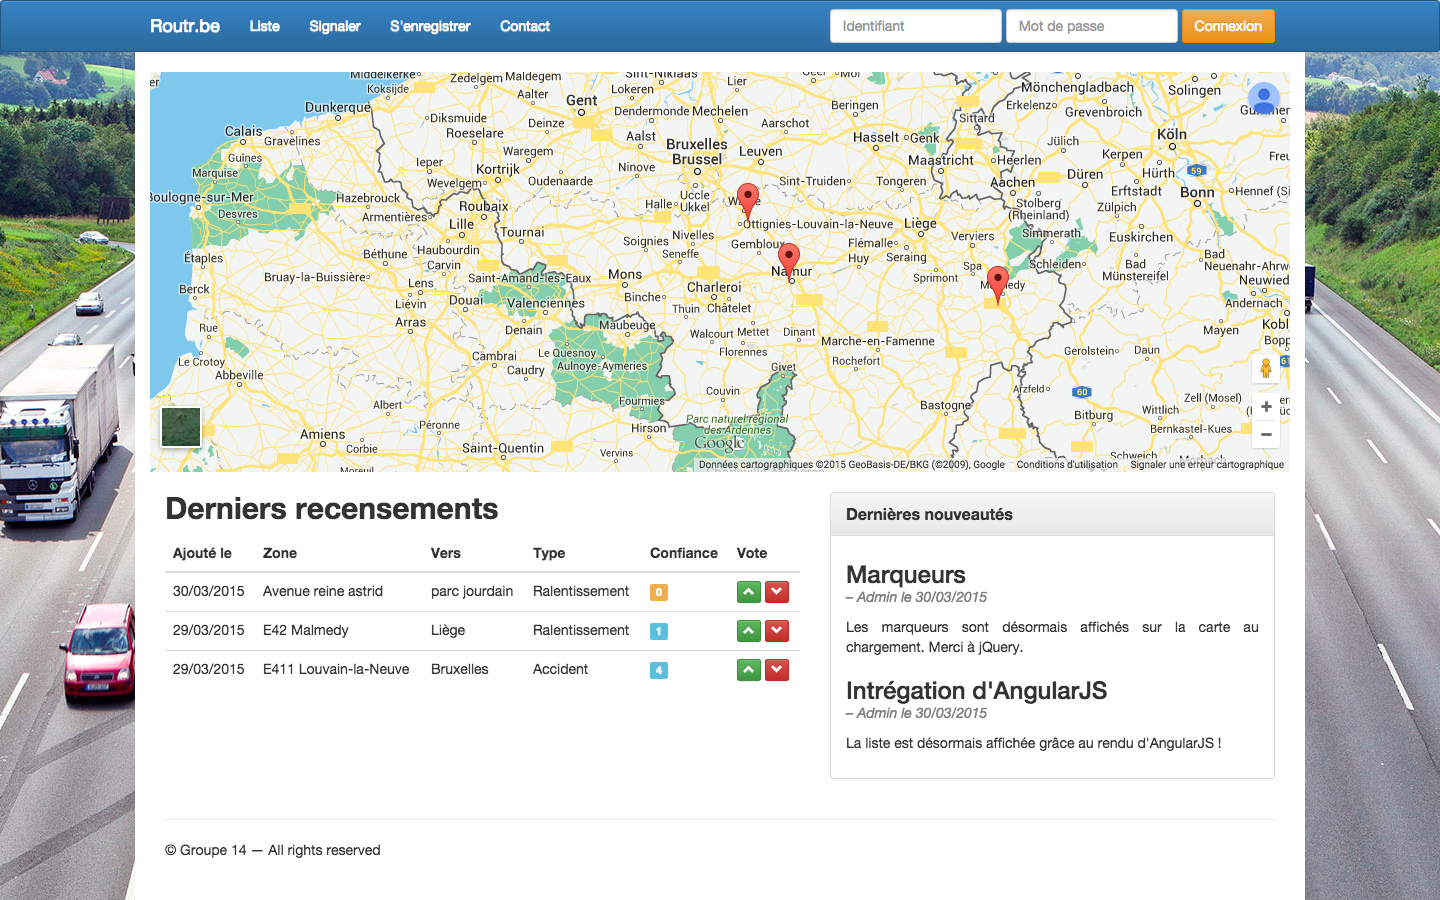
\includegraphics{main.png}}
\end{center}

\section{Analyse}

Notre application web étant fortement orientée sur la participation des utilisateurs, il est important de lister les besoins de celui-ci tel que :

\begin{enumerate}
	\item Un utilisateur peut facilement signaler un dérangement.
	\item Un utilisateur peut facilement lister la totalité des dérangements.
	\item Un utilisateur doit pouvoir trier la liste des dérangements afin d'en extraire ceux qui l'intéresse.
	\item Un utilisateur peut créer un compte.
	\item Un utilisateur peut évaluer la véracité d'un signalement.
\end{enumerate}

\section{Conception}

Comme nous étions limité à une application de type \texttt{M.E.A.N.} (\textit{i.e.} \textsf{mongoDB-ExpressJS-AngularJS-NodeJS}), nous avons dû adapter sa conception aux conventions et au modèle de \texttt{M.E.A.N.}.\\

Pour la persistance des données, la solution \textsf{mongoDB} ne stockant que des documents dans des collections, nous avons modélisé cinq collections nécessaires à l'application:

\begin{desclist}{\sf}{\rm$\;$\hfill--}[comments]
	\item[comments] Contient les commentaires sur un signalement.
	\item[news] Contient des articles d'actualités pour la page d'accueil.
	\item[sessions] Contient les sessions actives des utilisateurs connectés
	\item[signals] Contient les signalements.
	\item[users] Contient les utilisateurs
\end{desclist}

Chacune des ces collections possède un modèle correspondant afin de gérer les intéractions avec les données. Notre application ne génère pas d'objet telle qu'une application générique en POO le ferait mais au lieu de cela, travaille directement dans les documents de la base de données au travers des fonctions implémentées. Ce design lie très fortement les performances de notre application à celles du gestionnaire de base de données (\textit{i.e.} \textsf{MongoDB}).\\

L'architecture de l'application est de type MVC standard. Nos modèles de données sont stockés dans le dossier \textsf{models/}, nos vues dans le dossier \textsf{views/} et nos contrôleurs sont combinés avec les routes dans le dossier \textsf{routes/}.\\

Lorsqu'une requête est effectuée sur le serveur généré par \textsf{Express}, elle est captée par le fichier principal \texttt{app.js} qui redirige suivant la requête reçue vers la fonction correspondante dans un fichier du dossier \textsf{route/} défini. Ce fichier se charge avant tout d'ouvrir une connection à la base de données \textsf{mongoDB} en chargeant les collections qui lui seront nécessaires. Selon la fonction sélectionnée, et suivant la requête \textsf{http} reçue, une requête à la base de données sera effectuée et le résultat obtenu sera chargé dans une vue avant d'être renvoyé par Express au commandidaire de la requête \textsf{http}.

Cette architecture est simple et suffisamment efficace pour l'ordre de grandeur dans lequel l'application sera utilisée.
\section{Réalisation}

\subsection{Le système de vote}

Nous désirions un système de vote sous la forme d'un $+1$/$-1$ en \textit{single page} (\textit{i.e.} qui n'aurait pas besoin de recharger la page). Ceci était l'un de nos plus grand défi. Pour cela, \texttt{jQuery} est venu à notre aide. Nous n'avions jamais effectué de requête Ajax mais nous savions que c'était la technique à utiliser pour implémenter notre système de vote.

De ce fait, un pression sur une flèche de vote entraine l'exécution d'une requête ajax post sur le site et en fonction du code \textsf{http} retourné, nous pouvons savoir si le vote a été pris en compte ou non. Cela peut arriver si l'utilisateur n'est pas connecté ou qu'il a déjà voté. Une fois un vote pris en compte, le compteur est dynamiquement mit à jour sur le signalement.\\

\begin{figure}[!h]
	\centering
	\scalebox{0.7}{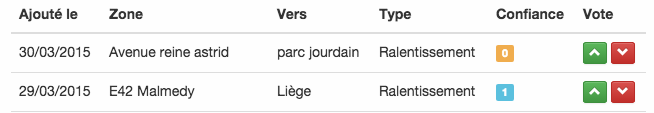
\includegraphics{vote.png}}
	\caption{Signalement avec le système de vote.}
\end{figure}

\pagebreak
\subsection{Le filtrage dynamique}

\begin{figure}[!h]
   	\begin{minipage}{0.6\linewidth}
\parindent 5mm Afficher tous les signalements est bien, mais pouvoir les trier est encore mieux. Malheureusement ce ne fut pas une chose aussi aisée que voulu car nous souhaitions que le filtrage soit dynamique. Dans le web de demain, il ne faut plus charger une page plus d'une fois. Pour cela, nous avons eu recours à \textsf{AngularJS}. Le framework expert dans les applications de type \textit{single page}. L'utilisation des filtres étaient parfaite pour filtrer dynamiquement la liste. Malheureusement, le moteur de rendu utilisé dans notre application Express ne nous permettait pas de passer directement des objets JSON au javascript côté client. Nous avons dû effectuer une requête Ajax pour recevoir la liste des signalements afin de la charger dans AngularJS. De là, un bug est apparu. AngularJS étant un mastodonte à charger, ainsi que Google Maps, il est strictement nécessaire qu'Angular se charge avant Google Maps pour afficher les marqueurs sur la carte à la page générale des signalements. De notre expérience, ce bug apparait en moyenne lors d’un chargement sur quatre de la page.
   	\end{minipage}
	%%%%%%%%%%%%%%
   	\begin{minipage}{0.4\linewidth}   
   		\centering
		\scalebox{0.5}{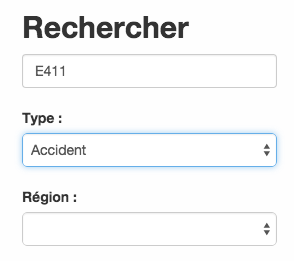
\includegraphics{filtrer.png}}
		\caption{Le filtrage.}
   	\end{minipage}  
\end{figure}

\subsection{La google maps}

Un site de signalement routier sans une carte n'est pas sérieux. C'est pourquoi nous avons intégré l'API javascript de google maps à notre application. Les lieux sont géolocalisés par leur zone, c'est pourquoi une description trop élémentaire telle que <<Le Ring>> pourrait entrainer le placement d'un marqueur à la mauvaise position.

\begin{figure}[h!]
	\centering
	\scalebox{0.25}{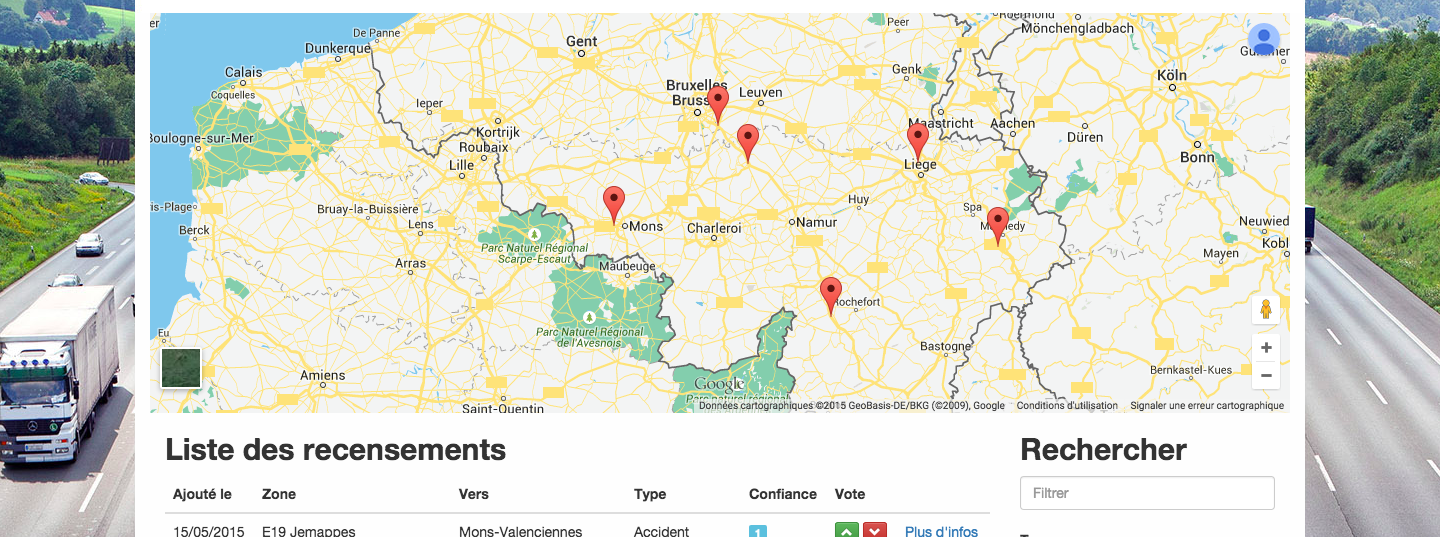
\includegraphics{gmap.png}}
	\caption{La google maps.}
\end{figure}

\subsection{Les commentaires}

\begin{figure}[H]
	\begin{minipage}{0.4\linewidth}   
    	\centering
		\scalebox{0.45}{
\includegraphics{comments.png}}
		\caption{Les commentaires.}
   	\end{minipage}
   	%%%%%%%%%%%%%
   	\begin{minipage}{0.6\linewidth}
\parindent 5mm Chaque signalement possède sur sa page d'information conrespondante, une section permettant aux utilisateurs connectés d'y placer un commentaire. Le champs permettant d'y ajouter un commentaire ne s'affiche que si l'utilisateur est connecté mais tous les visiteurs peuvent lire ceux déjà disponibles. Les commentaires sont classés du haut vers le bas dans l'ordre chronologique croissant, c.-à-d. que les plus récents se trouvent au dessus. Nous avons remarqué par présentation que cela peut perturber certains visiteurs du fait que le champ permettant d'insérer un commentaire se trouve en bas de la liste.
   	\end{minipage}
\end{figure}

\section{Choix d'implémentation}

Le projet fournit ne dispose pas d'une interface administrateur. Ceci fut un choix car une analyse de la tâche permettait d'affirmer que son implémentation ne serait qu'une suite de requêtes à la base de données pour les afficher dans des champs. Il n'y aurait aucun défi et donc aucun bénéfice éducatif. Ce choix pose malheureusement la difficulté que le seul moyen d'ajouter des messages d'actualité à la page d'accueil doit se faire à la main dans la base de données.

\section{Intégration continue}

Pour garder une trace du développement, nous avons décidé d'utiliser le système de contrôle de versions \texttt{Git} hebergé sur le site \texttt{github.com} (figure \ref{github}). Ceci nous a permis de découvrir une variété de services offerts par différentes plateformes pour automatiser et faciliter le développement d'applications Node.js. Cette approche appelée \textit{Continuous Integration} nous a permis en autre de vérifier automatiquement les dépendances de notre application grâce à la plateforme \texttt{David-dm.org} qui se charge de lire le \texttt{package.json} de notre application. Et nos tests ont pu eux aussi être automatisé par la plateforme \texttt{Travis-CI.com} (figure \ref{travis}). À chaque push effectué sur notre repo hebergé sur \textsf{Github}, \textsf{Travis} se charge de lancer nos tests déjà rédigés sur la dernière version hebergée et nous avertit par email quand un commit faissait passer le statu du projet de \textsf{compilable} à \textsf{générateur d'erreurs}. Des screenshots de l'utilisations de ces services sont disponibles en annexe.

\section{Conclusion}

L'application que nous avons developpée ce quadrimestre est un mélange de tout ce que le développement web d'aujourd'hui peut nous offrir. En combinant \textsf{mongodb}, \textsf{Express}, \textsf{AngularJS} et \textsf{NodeJS}, nous avons pu concevoir un site moderne dans la mode du genre \texttt{M.E.A.N.}
Cette plongée dans la pointe de la nouveauté nous aura mieux que jamais permis de plonger les mains dans cette branche très populaire de l'informatique qui a devant elle un long avenir et nous en sommes reconnaissants.

\pagebreak

\section{Annexe}

\begin{figure}[!ht]
\centering
\scalebox{0.3}{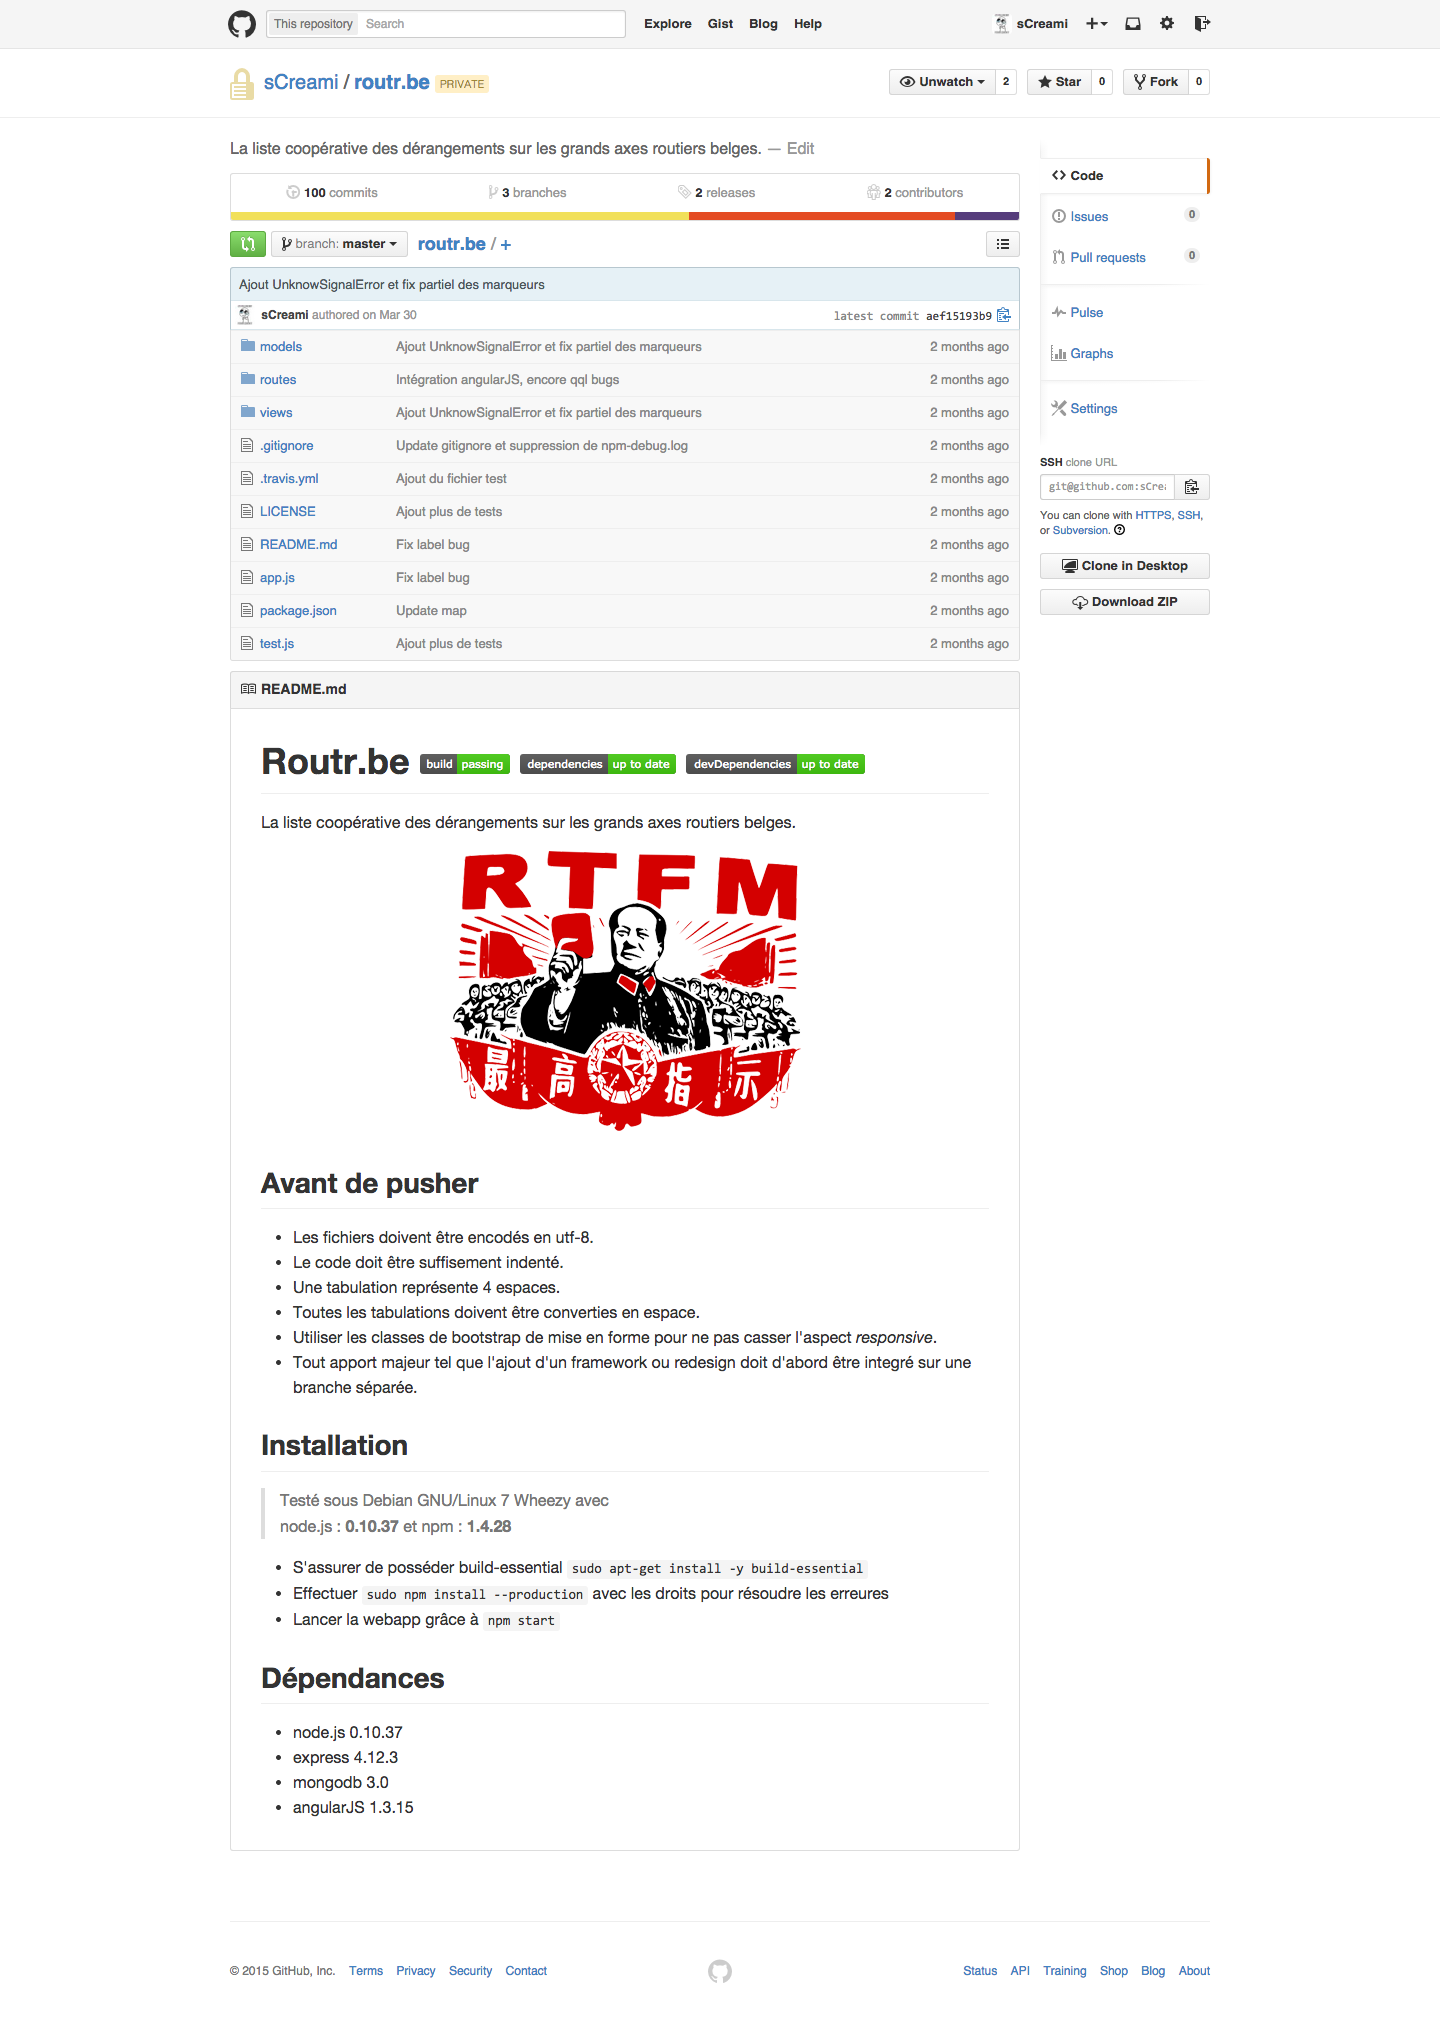
\includegraphics{github.png}}
\caption{routr.be sur github.com.}
\label{github}
\end{figure}

\begin{figure}[!ht]
\centering
\scalebox{0.34}{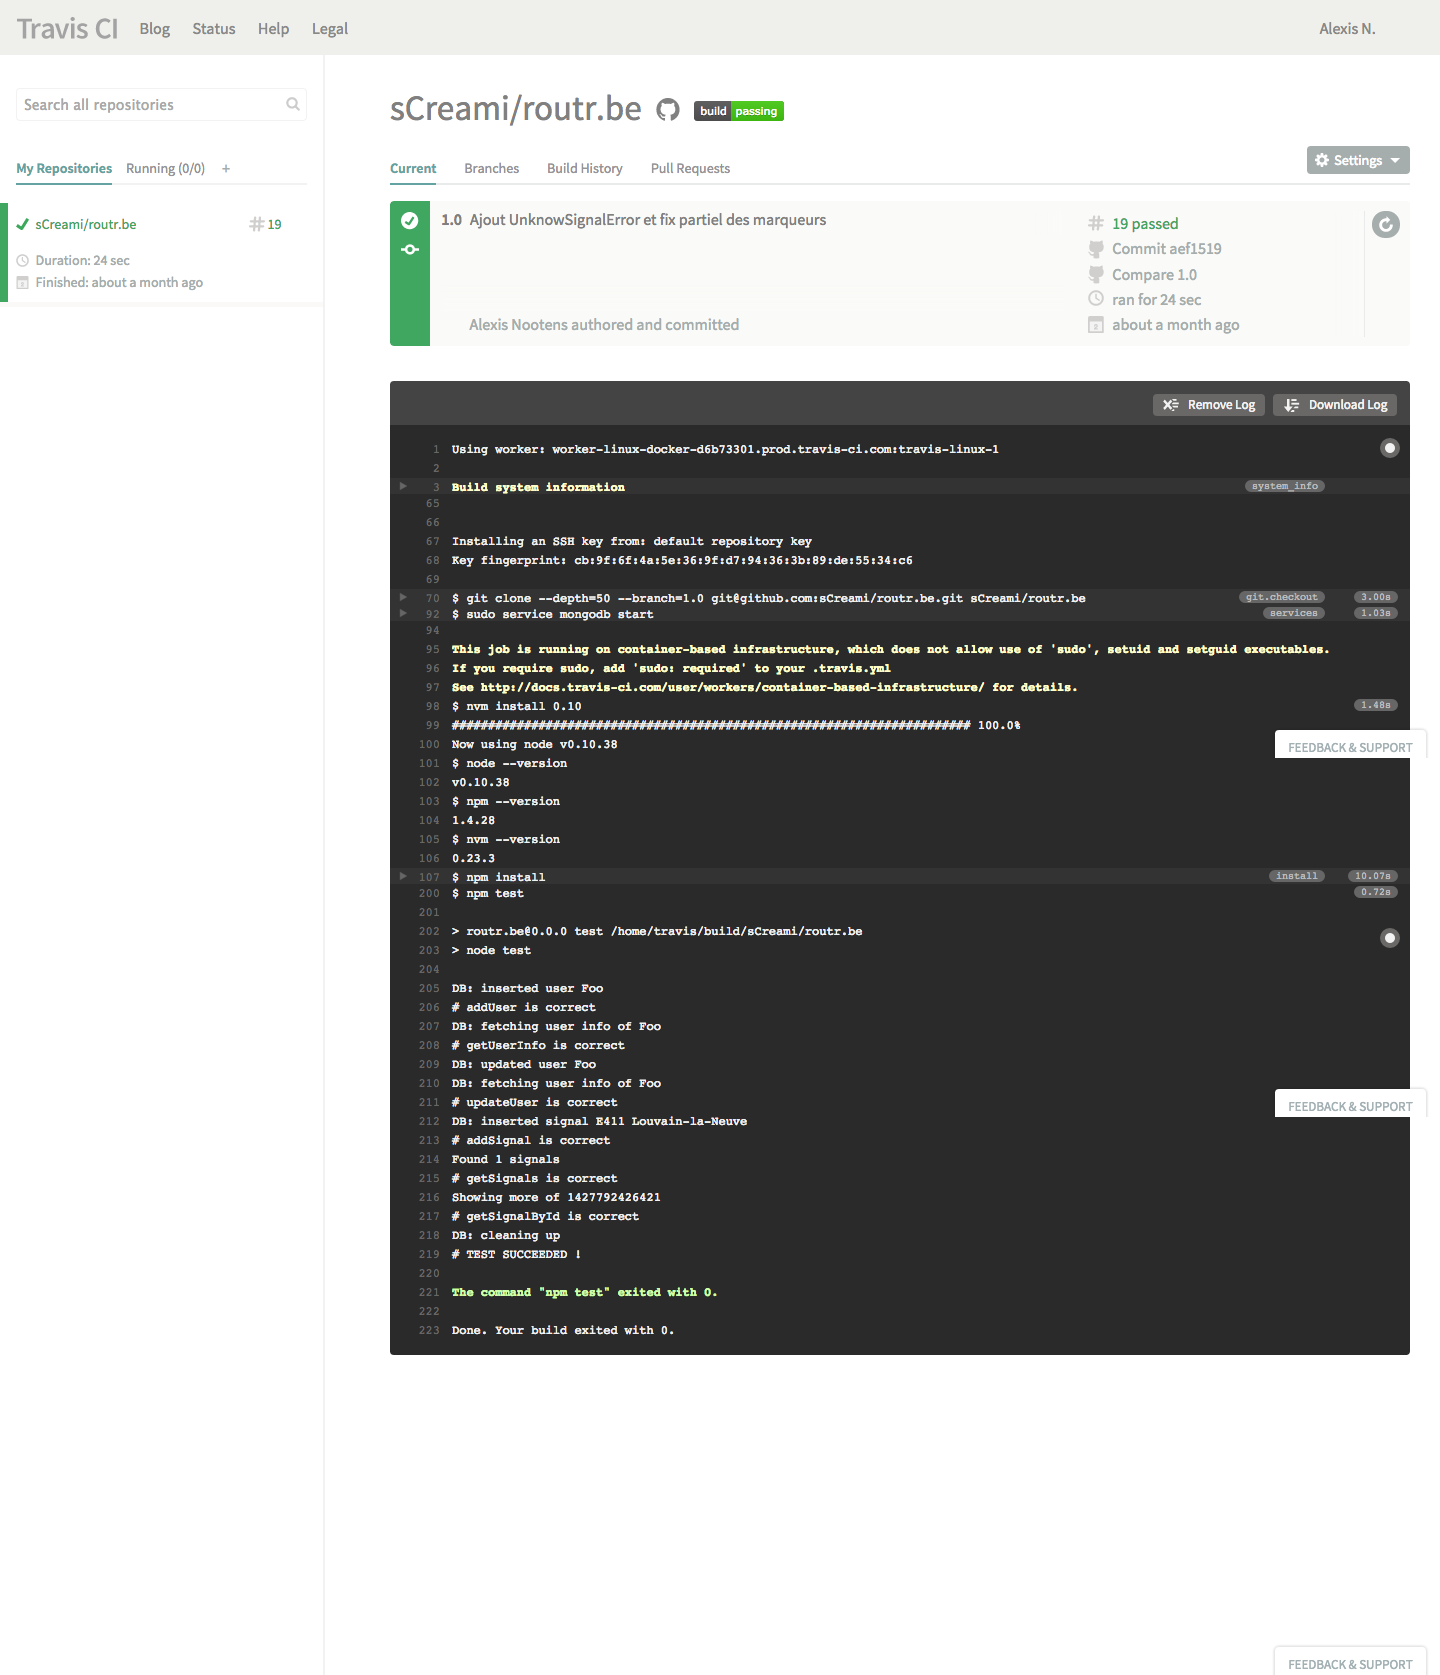
\includegraphics{travis.png}}
\caption{routr.be sur travis-ci.com.}
\label{travis}
\end{figure}

\end{document}